\documentclass[a4paper]{book}

\usepackage{ardour,graphicx,afterpage,url,xstring,xcolor}

% XXX: format
\newcommand{\button}[1]{#1}
\newcommand{\menu}[1]{\emph{\StrSubstitute{#1}{,}{ $\rightarrow$ }}}
\newcommand{\key}[1]{\emph{\StrSubstitute{#1}{,}{ + }}}

\newcommand{\screenshot}[3]{%
\begin{figure}[ht]%
\begin{center}
\includegraphics[scale=0.5]{screenshots/#1}
\end{center}
\caption{#2}
\label{#3}
\end{figure}}

% Voodoo from http://answers.google.com/answers/threadview?id=282787
\definecolor{ListingGrey}{rgb}{0.8,0.8,0.8}
\makeatletter\newenvironment{listing}{%
   \medskip\begin{lrbox}{\@tempboxa}\begin{minipage}{\columnwidth}\ttfamily}{\normalfont\end{minipage}\end{lrbox}%
   \colorbox{ListingGrey}{\usebox{\@tempboxa}}\medskip%
}\makeatother

\title{Ardour 3 --- A users' manual}
\author{The Ardour Community}
\date{}
\begin{document}

\maketitle

\tableofcontents

\chapter{Introduction}

Hello, and welcome to Ardour!

\section{What is Ardour?}

Ardour is an open-source digital audio workstation (DAW) for Linux and Mac OS~X.

\section{Typographical conventions}

This manual takes a cue from the \TeX{}book and uses special symbols
to denote sections which contain advanced material.  The reader can
skip these sections without any great loss.

\begin{danger}
Tricky parts of the text are marked with a `bend in the road' marker.
They contain extra information which may be of interest to advanced
users.
\end{danger}

\begin{ddanger}
Especially tricky parts of the text are marked with a double
bend-in-the-road marker.  Such sections will only be of interest to
the completist or serious hacker.
\end{ddanger}


\section{About this manual}

This manual is a constantly-evolving work-in-progress.  Any
suggestions for improvements, content, or comments on parts that do
not make sense are welcome to \url{cth@carlh.net}.  

\begin{danger}
For those familiar with `git', the manual's \LaTeX\ source can be
obtained from the git repository linked from
\url{http://carlh.net/ardour}.  Patches to the manual are most welcome.
\end{danger}


\chapter{Overview}

As one might expect, Ardour is similar in many ways to many other DAWs
and also has its fair share of differences.  This chapter gives an
overview of Ardour.


\section{JACK}

Ardour is built on another piece of software called JACK\footnote{JACK
  stands for the JACK Audio Connection Kit; a pleasingly recursive acronym}.
JACK has two main functions; first, it moves audio and MIDI to
and from a sound card, and second, it allows audio and MIDI to be
routed between different applications.

JACK provides a great deal of flexibility and power, especially when
running other applications (such as soft-synthesizers or samplers) at
the same time as Ardour.  It is somewhat similar to Steinberg's Rewire
technology, though broader in scope.  It is even possible to use JACK
to route audio and MIDI over network connections.

JACK is so important to Ardour's operation that it earns its own
discussion in chapter~\ref{ch:jack}.


\section{Sessions}

An Ardour \emph{session} is a container for an entire project.  A
session may contain an arbitrary number of tracks and busses
consisting of audio and MIDI data, along with information on processing
those tracks, a mix of levels, and everything else related to the
project.  A session might typically contain a song, or perhaps an entire
album or a complete live recording.

Ardour sessions are held in directories; these directories contain one
or more \emph{session files}, some or all of the audio and MIDI data
and a number of other state files that Ardour requires.  The session
file describes the structure of the session, and holds automation data
and other details.

\begin{danger}
Ardour's session file is kept in XML format, which is advantageous as
it is somewhat human-readable, and human-editable in a crisis!  Sound
files are stored in one of a number of optional formats, and MIDI
files as SMF (standard MIDI format).

It is also possible for Ardour sessions to reference sound and MIDI
files outside the session directory.
\end{danger}

Ardour has a current session at all times; if Ardour is started without
specifying one, it will offer to load or create one.



\section{Tracks}

A track is a concept common to most DAWs, and used also in Ardour.
Tracks can record audio or MIDI data to disk, and then replay it with
processing.  They also allow the audio or MIDI data to be edited in a
variety of different ways.

In a typical pop production, one might use a track each for the kick
drum, another for the snare, more perhaps for the drum overheads and
others for bass, guitars and vocals.

Ardour can record to any number of tracks at one time, and then play
those tracks back.  On playback, a track's recordings may be processed
by any number of plugins, panned, and its level altered to achieve a
suitable mix.

\begin{danger}
A track's type is really only related to the type of data that it
stores on disk.  It is possible, for example, to have a MIDI track
with a synthesizer plugin which converts MIDI to audio.  Even though
the track remains `MIDI', in the sense that its on-disk recordings are
MIDI, its output may be audio-only.
\end{danger}


\section{Regions}

A track may contain many segments of audio or MIDI\@.  Ardour contains
these segments in things called \emph{regions}, which are
self-contained snippets of audio or MIDI data.  Any recording pass,
for example, generates a region on each track that is enabled for
recording.  Regions can be subjected to many editing operations; they
may be moved around, split, trimmed, copied, and so on.


\section{Playlists}

The details of what exactly each track should play back is described
by a \emph{playlist}.  A playlist is simply a list of regions; each
track always has an active playlist, and a track's current playlist
can always be changed.


\section{Busses}

Busses are another common concept in both DAWs and hardware mixers.
They are similar in many ways to tracks; they process audio or MIDI,
and can run processing plugins.  The only difference is that their
input is obtained from other tracks or busses, rather than from disk.

One might typically use a buss to collect together the outputs of
related tracks.  Consider, for example, a 3-track recording of a
drum-kit; given kick, snare and overhead tracks, it may be helpful to
connect the output of each to a bus called `drums', so that the
drum-kit's level can be set as a unit, and processing (such as
equalisation or compression) can be applied to the mix of all tracks.


\chapter{JACK}
\label{ch:jack}

\section{Introduction}

JACK is the JACK audio connection kit.  It is a piece of software that
provides the low-level `plumbing' which allows Ardour to work.  Its
setup is crucial to Ardour; Ardour will not work without it.

JACK's essential task is to route audio and MIDI data to and from a
sound card, and also between applications.  It manages a set of
\emph{ports}, which it can connect together in arbitrary ways.
Figure~\ref{fig:typical-jack-session} gives a diagram of a moderately
complex JACK session.

\url{jackaudio.org/pulseaudio_and_jack}

\begin{danger}
JACK is not limited to the standard concept of the `sound card'.  You
-may choose to have no sound card at all (in which case JACK can run in
`dummy' mode).  It is also possible to send signals to and from JACK
over TCP/IP networks using netjack.  For simplicity, this manual will
assume that the user has a sound card in the conventional sense.
\end{danger}

\subsection{JACK and other audio software}

JACK is designed so that it uses a single sound-card, and has
exclusive control of that sound-card while it is running.  This is a
couple of consequences.  Firstly, if the sound card used to capture
audio is different from the one used to play it back, complications
arise.  Secondly, other software which tries to obtain exclusive
control of your sound-card, most notably `pulseaudio', may interfere
with JACK's operation.

\subsubsection{JACK with multiple sound cards}
\label{sec:jack-multiple-cards}

If at all possible, it is a good idea to use JACK with a single sound
card.  Correctly using more than one card at the same time is
difficult.  The main reason for this difficulty is that JACK assumes
that all sound cards and programs that it is connecting are running
with synchronised sample clocks.  Arranging this is not easy if there
are two cards; there will be two unsynchronised sample clocks.

If you accept that using multiple sound cards is not going to make
your life easy, and you want to do it anyway, there are a number of
approaches:

\begin{enumerate}

\item Use the \texttt{alsa\_in} and \texttt{alsa\_out} clients (Linux and ALSA only)

If you are using JACK on Linux and want to use additional devices that
have ALSA driver support (i.e. most PCI, USB and Bluetooth devices),
then this is the best option.

\texttt{alsa\_in} and \texttt{alsa\_out} are two clients written by
Torben Hohn that make a single ALSA device appear as a set
of JACK ports. They both use Erik de Castro Lopo's libsamplerate
library to do any resampling required to keep the audio in sync as the
clocks of each device drift over time.

To use them, you start JACK as normal. Then you start an instance of
\texttt{alsa\_in} or \texttt{alsa\_out} for each additional device
(and `direction') that you want to use. \texttt{alsa\_out} will create
a set of ports representing the playback capabilities of the device,
and \texttt{alsa\_in} will represent the capture/recording
capabilities. These two clients must be run inside a terminal window; 
there is no GUI for either of them. They both take arguments very much
like those of the JACK ALSA backend, with some additional controls
that affect the way that resampling is done. Full details are
available in the manual pages for each client, which you can read in a
terminal window with the command

\begin{listing}
man alsa\_in
\end{listing}

This page covers both clients, since their arguments are identical.

Note that you can use these clients even if you are running JACK with
a FFADO-supported device. The requirement for ALSA support only
applies to the extra devices you want to use, not the one that JACK
itself is using.

\item Use the JACK2 audio adapter(s) (Jack2 only)

% XXX More information is needed on this option

\item Using OS facilities to merge devices into a single pseudo-device

Both OS~X and Linux provide ways to configure your machine so that it
appears to have a new audio device that is actually a combination of
one or more real devices. You can use this approach to create the
configuration you want to use and then start up JACK using that new
`pseudo' device.

\begin{itemize}
\item OS X

You must perform these steps as a user with administrative
priviledges. The first thing to do is to open up
\menu{Applications,Utilities,Audio/MIDI Setup}. Go to the main menu
bar, click on \button{Audio} and then select \emph{Open aggregate device
editor}. Follow the simple instructions to add the each desired
playback or capture device to your new aggregate device. Then pick a
name for the new device. This is the name you will also use to choose
the device for use with JACK\@.

Note that there are quite a few subtle bugs with Apple's `aggregate
device' facilities. Various things can happen that will cause the
device to lose all of its playback channels or all of its capture
channels, for example. If this happens, it is generally necessary to
close all applications that are using any audio devices, and quite
often a reboot is required.

Starting with JACK2 version 1.9.6, the CoreAudio backend can now
dynamically create `aggregate devices' when needed (like when the -C
and -P arguments are used to specify the separated input and output
devices).

\item Linux

You will need to use a text editor to create or add to your
\texttt{~/.asoundrc} file. This file is read by any ALSA application
(including JACK, if its using the ALSA backend) and can be used to
define pseudo-devices of many different kinds. The key idea here is
that you're going to define a new pseudo-device composed of 2 or more
other devices. In our example, we'll just focus on 2 devices being
merged into 1, where both devices have just 2 channels in and
out. This is the text you need to make sure is in \texttt{~/.asoundrc} (below,
we describe what this does):

\begin{listing}
pcm.merge \{\\
    type multi;\\
    slaves.a.pcm hw:0\\
    slaves.a.channels 2;\\
    slaves.b.pcm hw:1\\
    slaves.b.channels 2;\\
    bindings.0.slave a;\\
    bindings.0.channel 0;\\
    bindings.1.slave b;\\
    bindings.1.channel 0;\\
    bindings.2.slave a;\\
    bindings.2.channel 1;\\
    bindings.3.slave b;\\
    bindings.3.channel 1;\\
\}\\
\end{listing}

Lets see what this does:

\begin{itemize}

\item It defines a new audio pseudo-device called `merge'. You can use
  this name anywhere you might use the name of an ALSA audio device,
  such as \texttt{hw:0} or \texttt{hw:HDA} or \texttt{hw:DSP} or
  \texttt{plughw:1}.
\item It names \texttt{hw:0} as the first component (or `slave') of
  this pseudo-device (\texttt{slave.a.pcm}) and \texttt{hw:1} as the
  second component (\texttt{slave.b.pcm})
\item It states that the pseudo-device will use 2 channels from the
  first component and 2 channels from the 2nd component.
\item The lines containing \texttt{binding.} list, in order, which
  channel of which component will correspond to the 4 channels of the
  pseudo-device. In the mapping shown above, the first channel comes
  from the first component, then the 2nd channel from the 2nd
  component, the 3rd from the first component and the 4th from the
  second component.

\end{itemize}

Note that numbering of devices and channels in ALSA starts at zero,
not one.

The most important and complex part of the above definition is the
channel mappings defined by the bindings lines. A full channel mapping
definition consists of a pair of a lines of the following general
form:

\begin{listing}
bindings.CHANNEL\_OF\_PSEUDO\_DEVICE.slave SLAVE\_DEVICE\_THAT\_WILL\_PROVIDE\_THIS\_CHANNEL\\
bindings.CHANNEL\_OF\_PSEUDO\_DEVICE.channel CHANNEL\_OF\_SLAVE\_DEVICE\_THAT\_WILL\_PROVIDE\_THIS\_CHANNEL
\end{listing}

So the specific pair of lines:

\begin{listing}
bindings.0.slave a;\\
bindings.0.channel 0;
\end{listing}

mean that `channel 0 of the pseudo-device will correspond to channel 0
of the first slave device'. Obviously by playing with this definition
you can create all sorts of wierd and wonderful mappings from the real
physical device channels to the pseudo-device channels. You probably
don't want to do that, though. The example above shows the most common
example: take the first $N$ channels from the first device, and the
second $M$ channels from the second device.

In theory, the above is enough to define a new pseudo-device, but many
applications, including JACK's ALSA backend, also want to open a
"control device" associated with the audio playback device. This is
where they can find out (and possibly control) various hardware
parameters associated with the device. Unfortunately there is no way
to merge these together in the same way, so we have to provide a
"dummy" control device definition that will keep such applications
happy. This definition looks like this:

\begin{listing}
ctl.merge \{\\
    type hw\\
    card 0\\
\}
\end{listing}

Notice that name following the \texttt{ctl.} text must be the same as
the name following \texttt{pcm.} in the device definition above. The
control device definition we've given here effectively means `if you
want to open the control device associated with ``merge'', open the
control device associated with the first installed audio/MIDI
device'. This probably isn't right of course --- `merge' involves two
cards --- but it will generally work just fine.

You can use this same approach to merge more than 2 devices - the
resulting \texttt{pcm.DEVICE-NAME} specification will obviously
include more lines. You can also use different devices than we did
above, where we just used the first and second installed card.

Note that you are likely to be better off using \texttt{hw:CARD} device names,
rather than \texttt{hw:N} names, when defining a `multi' pseudo-device, as
explained here. But further note that if you are using multiple
instances of the same type of audio hardware (say, 4 RME Multiface
devices), you will have to use \texttt{hw:N} because every card will have the
same \texttt{CARD} name. In fact, with such hardware, it may be very
difficult to ensure that \texttt{hw:0} always refers to the same audio
interface, because there is no ALSA name that uniquely defines a
particular PCI slot. This is currently an unsolved problem when using
multiple identical devices. If you use PCI (or PCIe or PCIx or other
derivatives of PCI) devices, the chances are that the first card will
always be the same one, and so forth, so its not likely to be an
issue. If you use several identical USB devices, it may be a more
significant problem.

\item Using the \texttt{-P} and \texttt{-C} arguments to a JACK backend

Several JACK backends, including the ALSA, FFADO and CoreAudio
versions, support the \texttt{-P} and \texttt{-C} arguments that can
be used to specify two different devices, one for playback and one for
capture/recording. You cannot use this to merge multiple devices for
playback or capture. This approach will not do any clock drift
correction, so as the two devices drift over time, you may get
glitches in the audio stream. Nevertheless, it can be an easy if
unreliable way to set up JACK so that, for example, it records from a
USB microphone and plays back via a builtin audio device.

When using \texttt{-P} or \texttt{-C} to specify different devices, do
not use the \texttt{-d} argument (which specifies a single device) and
do not use the \texttt{-D} argument (which tells JACK to configure a
device for playback and capture).

\end{itemize}
\end{enumerate}

\subsection{Will my sound card work?}

For your sound card to work with JACK, must have a driver suitable for
the operating system that you are running on.  For Linux, this means
that your card must be supported by ALSA or FFADO; ALSA supports
drivers using a wide variety of interfaces, and FFADO is for firewire
soundcards only. 

The easiest way to check on ALSA compatibility is to visit
\url{http://www.alsa-project.org/main/index.php/Matrix:Main}.  This is
the ALSA soundcard matrix and describes ALSA's support for a variety
of cards.  For FFADO, consult
\url{http://www.ffado.org/?q=devicesupport/list}.


\subsection{JACK versions}

For historical reasons, there are two `branches' of JACK that are both
maintained, and can be used as drop-in replacements for each other.
JACK1 has version numbers like 0.121.3, and JACK2 (also known as
jackdmp) has version numbers like 1.9.8.  Both implementations have
their advantages and disadvantages.  It does not matter a great deal
which one is used.

% XXX: unless what?


\section{Starting JACK}

Ardour can start JACK automatically when it starts; and indeed many
users will find that this works perfectly well.  It is also possible
to start JACK manually, either at the command line or using a tool
such as QJackCtl\footnote{\url{http://qjackctl.sourceforge.net}} or
JackPilot\footnote{\url{http://www.jackosx.com}}.

\subsection{Parameters}

JACK has many parameters which affect its operation.  Some of the more
important ones are discussed here.

\subsubsection{Sampling rate}

This is the number of samples per second that JACK will process, and
is important as it will govern the sampling rate that all audio
applications will run at.  The chosen rate must be supported
by the sound card, so values such as 44.1kHz, 48kHz, 96kHz
et.\ cetera are typical choices.  The higher the sampling rate, the
higher the theoretical audio frequency that the system can reproduce,
but also the more disk space will be consumed by audio recordings, and
the more CPU power will be required to run audio plugins.

\subsubsection{Frames per period}

In a move necessary for efficiency, JACK does not process audio
sample-by-sample, but in blocks of samples.  The size of these blocks
can be selected when starting JACK\@.  If the frames per period count
is made smaller, the latency experienced by sounds going into and
coming out of the computer will be reduced; on the other hand, smaller
buffers make the computer work harder, and may result in other
problems if the computer is not well set-up.  It is usually difficult
to get below 64 frames per period on a typical desktop computer, and
values as high as 2048 frames per buffer if you do not particularly
care about latency.

\begin{danger}
The frames per period value governs how often JACK will talk to the
sound card.  If, for example, JACK is set to 64 frames per period, the
sound card will tell JACK when it has 64 new frames ready; JACK must
then respond before the next 64 frames arrives.  This has the
consequences that JACK is awoken more often, causing a greater CPU
load, and that the requirements for JACK's response time are much more
critical with smaller period sizes.  Some systems will struggle to wake
JACK up in time, making larger period sizes more reliable on those systems.
\end{danger}

\subsubsection{Number of periods}

This is value related to the frames-per-period value above; 2 is
typical, and will work for most sound cards and systems.  It is worth
trying 3 here if problems are experienced.


\section{Troubleshooting JACK}

\subsection{I am getting lots of xruns!}

An \emph{xrun} is JACK's way of saying that the sound card wanted
attention, but JACK could not provide it quickly enough.  The causes
of xruns are many and various.  The remainder of this section lists
some common causes of xruns.


\subsubsection{Buffer size or period count too small}

The JACK `buffer size', or number of frames per period, governs how
often JACK has to talk to the sound card; smaller buffer sizes require
JACK to communicate with the sound card more often and with tighter
deadlines.  Increasing buffer size can be a simple way to reduce
xruns.

Similarly, if you have a lot of xruns, particularly with a USB device,
try increasing JACK's period count from 2 to 3.


\subsubsection{JACK not running with real-time priviledges}

JACK will try, by default, to obtain \emph{real-time} scheduling
priviledges when it starts.  If it suceeds, it means that the
operating system will treat JACK as higher priority than some other
tasks when it needs to talk to the soundcard, which is very likely ton+
reduce the incidence of xruns.

JACK may fail to obtain real-time priviledges.  This is usually
because the operating system does not, by default, allow it, and so
its configuration must be altered.  For Debian- and Ubuntu-based
distributions, the best way is usually to add your user to the `audio'
group using

\begin{listing}
usermod -a -G audio fred
\end{listing}

where \texttt{fred} is your user ID\@.  After this, configure the audio
group to be allowed appropriate settings by editing
\texttt{/etc/security/limits.conf} and adding

\begin{listing}
@audio - rtprio 99\\
@audio - memlock unlimited
\end{listing}

to the bottom of of the file.  This allows members of the audio group
to start tasks with high real-time (RT) priority, and also allows them
to lock their memory into `real' memory; this is another step that
improves real-time performance.

After making these changes you will need to log out and log back in
again to see the effects.


\subsection{I can play back but I cannot record, or vice versa}

This is commonly caused by JACK's basic prediliction for using only
one sound card.  If you are using different sound cards for playback
and record (which will be the case even if you are doing playback via
HDMI and recording via an on-board sound-card) you will need to set
JACK up to use multiple sound cards, as discussed in
Section~\ref{sec:jack-multiple-cards}.


\chapter{Quick start}
% XXX: links to things later on

This chapter blithely assumes that you just want to use Ardour to make
a basic audio recording from a sound card, and describes how that can
be achieved.

\section{Starting Ardour and creating a session}

When Ardour is run for the first time, it starts with the dialogue box
shown in Figure~\ref{fig:welcome-to-ardour}.  Click \button{Forward} to continue.

\screenshot{welcome-to-ardour.png}{Welcome to Ardour!}{fig:welcome-to-ardour}

As it is the first run, Ardour now asks a few basic questions about
how it should be set up.  Its first question is about where to put
sessions by default, as shown in
Figure~\ref{fig:default-folder-for-new-sessions}.  The initial choice
will be the your home directory; other locations can be selected by
clicking on the button and selecting an alternative directory.

\screenshot{default-folder-for-new-sessions.png}{Default folder for new sessions}{fig:default-folder-for-new-sessions}

The next choice governs how Ardour will handle monitoring, as shown in
Figure~\ref{fig:monitoring-choices}.  For the purposes of this test,
choose `Ask Ardour to playback material as it is being recorded', as
this makes things slightly clearer in many cases.

\screenshot{monitoring-choices.png}{Monitoring choices}{fig:monitoring-choices}

Following this, Ardour asks for a choice with respect to a monitor
section (see Figure~\ref{fig:monitor-section}).  This is explained in
more detail later; for now, just choose the default `use a master bus
directly'.

\screenshot{monitor-section.png}{Monitor section}{fig:monitor-section}

At this point, if JACK has not already been started, Ardour will try
to do it for you.  In order to do that, it asks about how JACK should
be set up (Figure~\ref{fig:audio-midi-setup-device}).

There are three pages to the Audio / MIDI setup dialogue; the first is
`device', which allows selection of the sound card that Ardour will
use, the sampling rate at which it will operate, and the buffer size.
For now, select the interface that you are using for recording and
leave other options as they are.  For more information on the options
here, consult chapter~\ref{ch:jack}.

\screenshot{audio-midi-setup-device.png}{Audio/MIDI setup --- device}{fig:audio-midi-setup-device}

The final step in creating our session is to give it a name, as in
Figure~\ref{fig:new-session}.  Enter something like `test' and click
\button{Open}.  At last, the reward should be the editor window
(Figure~\ref{fig:editor}).  The session is created!

\screenshot{new-session.png}{New session}{fig:new-session}

\begin{figure}[ht]
\begin{center}
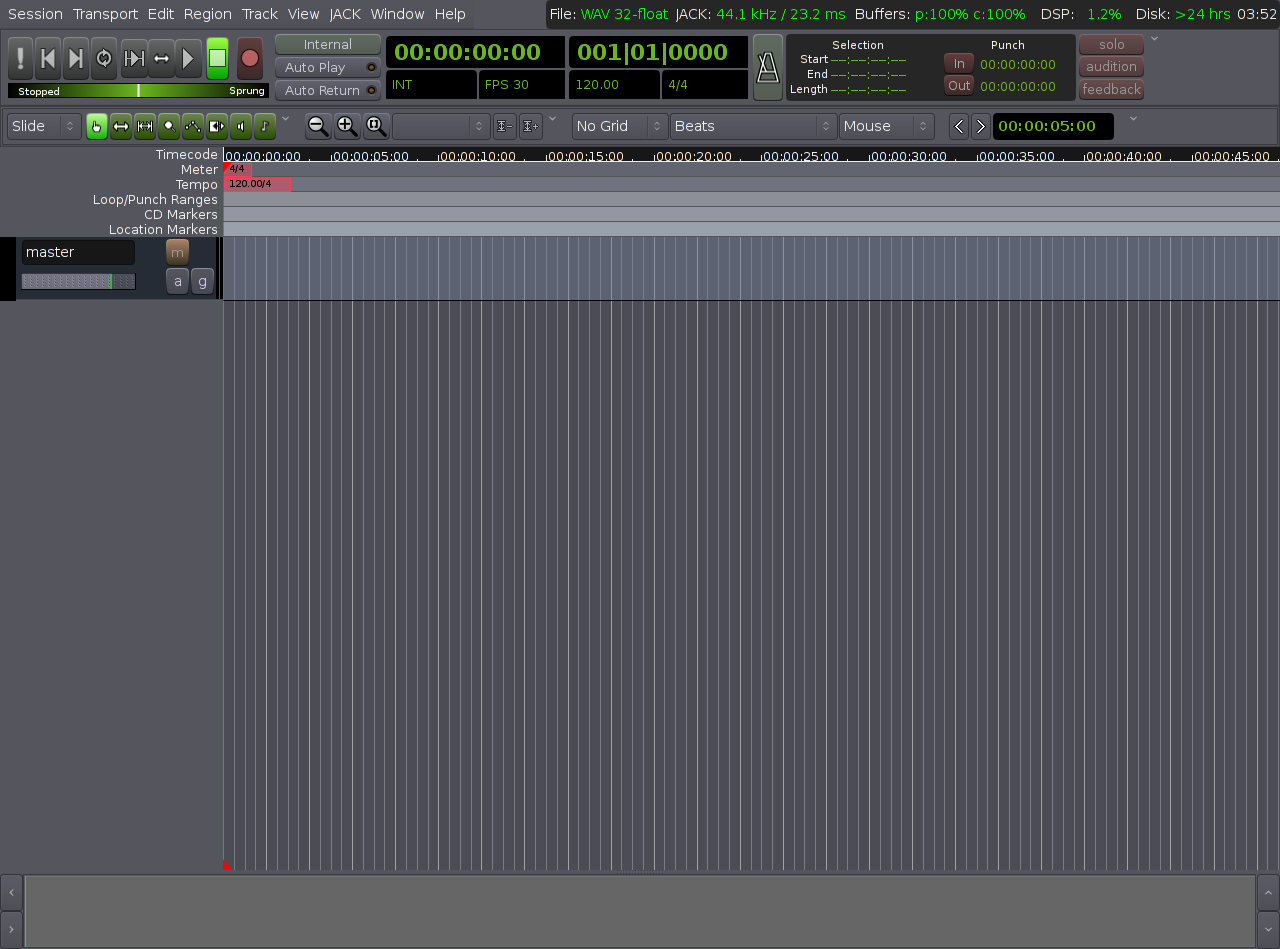
\includegraphics[scale=0.3]{screenshots/editor.png}
\end{center}
\caption{\ldots and finally: the editor!}
\label{fig:editor}
\end{figure}

\section{Adding a track and connecting it up}

The next step is to add a track to our session so that we have
something to record onto.  Choose \menu{Track,Add Track or Bus...}
from the menu at the top of the editor window.  This will bring up a
dialogue box, as shown in Figure~\ref{fig:add-track-or-bus}.

\screenshot{add-track-or-bus.png}{Add Track or Bus dialogue}{fig:add-track-or-bus}

For now, leave the options as they are; this will create a single
monophonic audio track.  This track must now be connected to the sound
card so that it can record incoming audio.

Perhaps the easiest way to connect up this new track is to open its
editor mixer strip.  Do this now by pressing \key{Shift,E} or
choosing \menu{View,Show Editor Mixer} from the main menu.  The top of
the mixer strip that appears looks like that in
Figure~\ref{fig:top-of-mixer-strip}.

\screenshot{top-of-mixer-strip.png}{Top part of a mixer strip}{fig:top-of-mixer-strip}

At the top of this mixer strip there are three main buttons.  The
first, labelled `Audio 1' (the name of the track) can be clicked on to
open a menu of options for the track.  The second, marked `1' is the
input selector, and the third, marked $\phi$, is a button to invert
the track's signal.

In order to look at the connections to the input of this track,
left-click on the button marked `1' to open the input \emph{port
  matrix}, as shown in Figure~\ref{fig:input-port-matrix}.

\screenshot{input-port-matrix.png}{Input port matrix}{fig:input-port-matrix}

The port matrix is the main interface that Ardour offers for
connecting things together.  In our example matrix, the left-hand side
shows a set of ports that generate audio data; these correspond to the
sound card inputs, outputs of Ardour busses and tracks, and other
things that may exist on the system.  Different groups of these ports
can be seen by choosing one of the tabs on the far left-hand side of
the dialogue.

At the bottom of the dialogue is the input to our track.

In the example matrix, there is a green dot at the intersection of the
`L' part of `in $1+2$' and the `Audio 1 in' port.  This means that the
input of the `Audio 1' track hardware input 1.  Change this
connection, if necessary, by clicking on the square which corresponds
to the input to record from.  At this point, the Audio 1 meter should
display any signal that is being sent into the sound card.  If this is
not working, something has gone wrong.

\section{Recording}

At this point, Ardour is receiving a signal from some external sound
source via the sound card.  It is now possible to make a test
recording.  Click the record-enable buttons (red buttons with a pink
circle) in both the `Audio 1' track controls and the main transport
controls (shown in Figures~\ref{fig:track-controls} and
\ref{fig:transport-controls} respectively.

\screenshot{track-controls.png}{Track controls area}{fig:track-controls}
\screenshot{transport-controls.png}{Main transport controls}{fig:transport-controls}




\section{Adding another track as an overdub}

\section{Mix-down}

\section{Export}


\chapter{Unfiled miscellany}

\section{The processor list}

% XXX: sshot



\section{Monitoring}

The basic role of a track is to record and playback audio or MIDI
data.  In some situations, however, it is useful to be able to get a
track to pass live audio or MIDI from its input to its output.
Consider, for example, a track with a couple of plugins that is being
used for a vocal recording.  It may be desirable to listen to the
processed live vocal from the output of the track, either before or
during recording.  Generally speaking, the passing of live input data
around Ardour is called \emph{monitoring}.


\subsection{Different ways of monitoring}

There are three basic ways in which monitoring may be approached:

\begin{itemize}
\item External monitoring --- this is where Ardour plays no role in
  monitoring at all.  Perhaps the recording set-up has an external
  mixer which can be used to set up monitor mixes, or perhaps the
  sound-card being used has some `listen to the input'-style feature.
  This approach often has the advantage of zero or near-zero latency.
  On the other hand it requires external hardware, and the monitoring
  settings are not saved with the session.

% XXX diagrams here

\item JACK-based `hardware' monitoring --- some sound cards have the
  ability to mix signals from their inputs to their outputs with zero-
  or low-latency.  Furthermore, on some cards these features can be
  controlled by JACK\@.  This is a nice arrangement, if the sound card
  supports it, as it combines the convenience of having the monitoring
  controlled by Ardour with the low latency operation of doing it
  externally.

\item Software monitoring --- this where all monitoring is performed
  by Ardour; it makes track inputs available at track outputs, under
  the influence of various controls.  This approach will almost always
  have more routing flexibility than JACK-based monitoring.  The
  disadvantage is that there will be a latency between the input and
  the output which will depend mainly on the JACK buffer size that is
  being used.

\end{itemize}

\subsection{Setting up monitoring}

There are three main settings which affect how monitoring is
performed.  The first is `Record monitoring handled by' in the
\emph{Audio} tab of the \emph{Ardour Preferences} dialogue.  There are
two or three options here, depending on the capabilities of your
hardware:

\begin{itemize}
\item \emph{ardour} --- Ardour handles monitoring itself (software monitoring).
\item \emph{audio hardware} --- Ardour does no monitoring at all, and
  assumes you will do it yourself (external monitoring)
\item \emph{JACK} --- Ardour will ask JACK to, in turn, ask the sound
  card to handle monitoring.  This option is only available if it is
  supported by your sound card (hardware monitoring).
\end{itemize}

The other two settings are more complex; one is `Tape machine mode',
in the same dialogue, and the other is `Monitoring automatically
follows transport state (``auto-input'')' setting in \emph{Session
  Properties}.

Monitoring is also somewhat dependent on the state of the track's
record-enable button, the session record enable button, and whether or
not the transport is rolling.


\subsection{Monitoring in software or hardware monitoring modes}

If Ardour is set to `external monitoring', the explanation of Ardour's
monitoring behaviour is simple: it does not do any.  In the other two
modes, things are more complex.


\subsection{Monitoring in non-tape-machine mode}

This section describes what happens when Ardour is \emph{not} set to
tape-machine mode.

Consider first the case when a track is record-enabled.  In this
situation, it will always monitor the live input \emph{unless} the
session is \emph{not} record-enabled, auto-input is enabled, and the
transport is rolling.  

When a track is not record-enabled, the track will play back its
contents from disc \emph{unless} the transport is stopped and
auto-input is enabled.  In this case, the track monitors its live
input.


\subsection{Monitoring in tape-machine mode}

In tape-machine mode, things are slightly simpler; when a track is
record-enabled, its behaviour is the same as in non-tape-machine mode:
it will always monitor the live input \emph{unless} the session is
\emph{not} record-enabled, auto-input is enabled, and the transport is
rolling.

When a track is not record-enabled, however, the track will always
just play back its contents from disk; the live input will never be
monitored.


% XXX some more rational explanation of why things are like this
% XXX metering!


\section{Tracks and busses in detail}

\begin{ddanger}
This section goes into somewhat unhealthy detail about how tracks and
busses operate internally.  It may be of interest to almost nobody.
\end{ddanger}

Tracks and busses in Ardour share a common basis; they are both
pathways through which audio and MIDI data can pass, experiencing
various processing and distribution along the way.  The only real
difference between a track and a bus is that a track can either obtain
its input from a JACK port, or from files on disk; a bus has no disk
files, so only processes signals coming from other parts of Ardour, or
from other programs via JACK\@.

Internally, Ardour uses the term `route' to describe a bus, with a
track being a superset of the route's functionality (to include the
parts which read from and write to disk).  This chapter uses the word
`route' to indicate either a track or a bus, where the two have the
same behaviour.

Not all of the processing that signals experience as they travel
through routes visible in the Ardour user-interface. The visible parts
are the plugins, the fader, the meter and (if present) the panner.
There are other invisible processes that happen to support Ardour's
internal operation.  Figure~\ref{fig:route-in-detail} gives a
representation of the entire pathway of a route.

% XXX: panning
\begin{figure}[ht]
\begin{center}
\includegraphics{diagrams/route-in-detail.pdf}
\end{center}
\caption{Detailed view of a route}
\label{fig:route-in-detail}
\end{figure}

Audio or MIDI data starts from either a set of JACK ports or a disk
file.  Busses always take their initial data from JACK ports, and
tracks can do either depending on monitoring settings.  It is possible
for tracks and busses to have no input, in which case the signal
starts off as silence.

If a track is recording, data is taken straight from the JACK input
ports and recorded; no processing on track will have any effect on the
recorded signal.

The signal then enters the processing chain.  Internally, this chain
is a set of `processors' connected in series.  

\subsection{Export}

% XXX

\subsection{Internal return}

This is the point at which internal send signals from other routes
appears in the route being sent to.  This processor gathers signals
from all its connected sends and mixes them with the signal in the
route at that point.

\subsection{Monitor control}

% XXX

\subsection{Monitor send}

The monitor send is an internal send which sends the route's signal,
whever it is located, to the monitor bus.  The monitor send is located
in different places, depending on the settings for AFL and PFL\@.

\subsection{Meter}

The meter processor passes signals unaltered, but meters them on the
way through.  It can be moved around depending on the meter point settings.

\subsection{User processors}

These are the `conventional' user-visible processors: plugins and
internal sends to other tracks or busses.

\subsection{Amp}

This is a basic gain-control element which is controlled by the fader.

\subsection{Main out}

This processor takes the route's signal, optionally pans it, and then
passes it to a set of JACK ports; this represents the main output of
the route.

\end{document}



